\documentclass[document]{xmgr}
% Jeśli nowe rozdziały mają się zaczynać na stronach
% nieparzystych:
%\documentclass[openright]{xmgr}

%\defaultfontfeatures{Scale=MatchLowercase}
%\setmainfont[Numbers=OldStyle,Ligatures=TeX]{Minion Pro}
%\setsansfont[Numbers=OldStyle,Ligatures=TeX]{Myriad Pro}
% for fontspec version < 2.0
\setmainfont[Numbers=OldStyle,Mapping=tex-text]{Arial}
\setsansfont[Numbers=OldStyle,Mapping=tex-text]{Times New Roman}
\usepackage{amsmath}
\usepackage{amsfonts}
\usepackage{listings} 
\usepackage{color}
\usepackage{graphicx}
\usepackage{float}
\usepackage[section]{placeins}



\setmonofont[Scale=0.75]{Monaco}

% Opcjonalnie identyfikator dokumentu
% drukowany tylko z włączoną opcją 'brudnopis':
\wersja   {wersja wstępna [\ymdtoday]}

\author   {Szymon Rękawek}
\nralbumu {206288}
\email    {rekawekszymon@gmail.com}

\title    {Gra Thuego}
\date     {01.01.2016}
\miejsce  {Gdańsk}

\opiekun  {prof. UG dr hab. T. Dzido}

% dodatkowe polecenia
%\renewcommand{\filename}[1]{\texttt{#1}}
\definecolor{stress}{cmyk}{0,1,0.13,0} % RubineRed
\definecolor{topic}{cmyk}{0.98,0.13,0,0.43} % MidnightBlue

\begin{document}

% streszczenie
\begin{abstract}
Celem pracy było zaprogramowanie gry opierającej się na twierdzeniach Axela Thue, na temat powtórzeń oraz nasunięć wewnątrz ciągu. Głównymi funkcjonalnościami aplikacji jest potyczka między dwoma graczami oraz symulacja przeprowadzona przez konkurujące ze sobą algorytmy. 

Powstały dwa warianty aplikacji, pierwszy z nich napisany został za pomocą silnika \textit{Unity3d}, posiada interfejs graficzny, nie ma jednak innego zastosowania niż bicie własnych rekordów. Drugi jest napisany w jęzku \textit{Java}, bez interfejsu graficznego, w zamian oferuje funkcjonalność dokonywania testów na serwerze zdalnym i zawiera wiele opcji konfiguracyjnych, między innymi precyzowanie poziomu \textit{inteligencji} algorytmów. 

Przeprowadzone badania wykazały, że algorytmy symulujące graczy działają prawidłowo i zwiększanie ich poziomu skutkuje lepiej podejmowanymi decyzjami. Na podstawie badań ustalona została maksymalna długość rozgrywki przy odpowiedniej taktyce, dla rozgrywek zawierających określoną ilość symboli z których tworzony jest ciąg.
\end{abstract}

% słowa kluczowe
\keywords{Thue, Java, ciąg, programowanie, Unity3d}

% tytuł i spis treści
\maketitle

% wstęp
\introduction

Tematem niniejszej pracy jest Gra Thuego. Axel Thue był norweskim matematykiem żyjącym w latach 1863 - 1922, znanym z prac z zakresu kombinatoryki.

Thue pracował nad problemami, powstałymi w wyniku badań nad sekwencjami symboli. Praca Thue \cite{repetition} opisywała problem, który autor nazwał \textit{nieredukowalne słowa} (\textit{irreducible words}). Poświęca w niej szczególną uwagę dwu i trzy literowym przypadkom. W skrócie wprowadza pojęcie znane obecnie jako \textit{Thue-Morse word} i pokazuje, że nieskończone słowa bez nasunięć (\textit{Overlap-free}) są pochodnymi tej sekwencji. W swoich pracach definiuje kolejną strukturę, a mianowicie infinite \textit{Square-Free word}, oraz przedstawia sposoby generowania nieskończenie długich słów wolnych zarówno od kwadratów jak i nasunięć.

Gra która powstała na podstawie teorii Thuego w skrócie polegała będzie na utworzeniu jak najdłuższego ciągu znaków nad określonym z góry alfabetem. Zależnie od trybu gry, kończyć się ona będzie w momencie gdy pojawi się zdefiniowany na początku rodzaj powtórzenia w tworzonym przez nas, bądź algorytm ciągu. Jednym z trybów gry jest walka komputera przeciwko niemu samemu, po takiej rozgrywce przedstawione zostaną złożoności czasowe oraz wnioski wynikające z obranej przez oponentów taktyki. 

Ostatnia część pracy poświęcona jest analizie algorytmów zarówno pod względem czasu ich wykonywania jak i zdolności do przewidywania ruchów przeciwnika. Badany jest również aspekt tego ile symboli z których tworzony jest ciąg, jest potrzebnych na rozegranie dostatecznie długiej rozgrywki, przy możliwie najdoskonalszej taktyce.

\chapter{Teorie Axela Thue na temat sekwencji symboli}
Zanim przejdziemy do twierdzeń, koniecznym jest wyjaśnienie podstawowych twierdzeń, które w dalszej części pracy będą wielokrotnie wykorzystywane. Niżej wyjaśnione zostały sposoby generowania nieskończenie długich ciągów składających się z dwóch symboli, nie zawierających nasunięć. Po czym ukazane zostały metody tworzenia nieskończenie długich ciągów na trzech znakach, wolnych od kwadratów. Na koniec części teoretycznej przedstawiony został pomysł gry dla dwóch graczy wykorzystujący powyższe własności.


\section{Definicje}


\begin{itemize}
\item Alfabet jest skończonym zbiorem symboli lub liter.
\item Słowo alfabetu $A$ jest skończoną sekwencją elementów z $A$. 
\item Długość słowa $\omega$ jest reprezentowana przez $|\omega|$.
\item Puste słowo o długości $0$ jest reprezentowane przez $\varepsilon$.
\item Czynnik (factor) słowa $\omega$ jest słowem $u$, które występuje wewnątrz $\omega$ formie $\omega = xuy$, podczas gdy $x$ oraz $y$ również są słowami tego alfabetu.
\item Kwadrat (square) jest słowem w formie $uu$, gdzie $u$ jest niepuste.
\item Square-free, słowo jest wolne od kwadratów, jeśli żaden z jego czynników nie jest kwadratem.
\item Nasunięcie (Overlap) jest słowem w formie $xuxux$, gdzie $x$ jest niepuste. Nazwa pojęcia wzięła się z tego, że $xux$ występuje dwa razy w $xuxux$. Pierwszy raz jako prefiks (początkowy czynnik) oraz jako sufiks (końcowy czynnik) i te dwa wystąpienia mają wspólną część - centralne $x$, a więc \textit{nasuwają} się na siebie.
\item Overlap-free - słowo w którym żaden z czynników nie nasuwa się na siebie.
W definicji Axela Thue słowo $\omega$ w alfabecie długości n jest nieredukowalne jeśli jakiekolwiek dwa wystąpienia tego samego słowa jako czynnik wewnątrz $\omega$ są zawsze oddzielone od siebie przez $n-2$ liter. Oznacza to, że nieredukowalne dwuliterowe słowo jest bez nasunięć i nieredukowalne trzyliterowe słowo jest bez kwadratów.
\item Morfizm - mapowanie obiektu z jednej matematycznej struktury w inną.
\end{itemize}



\section{Thue-Morse word}
Rozważmy nieskończone słowo

{\centering $01101001100101101001011001101001 ...$ \par}

Jest to słowo stworzone z dwuliterowego alfabetu, które nie zawiera ani jednego nasunięcia. Zostało ono nazwane po Thue, który badał jego właściwości w referacie z 1906 roku, oraz Morsie, który odkrył je na nowo w latach 20 XIX wieku. Słowo Thue-Morse'a występuje również o wiele wcześniej w wiadomościach  Prouheta \cite{prouhet} z Francuską Akademią Nauk w 1851 roku. Prouhet podał więcej ogólnych konstrukcji, uzyskując nie tylko słowo Thue-Morse'a, ale całą rodzinę słów na większych alfabetach mających inne interesujące właściwości. Słowa te czasami odnoszą się do ogólnych słow Thue-Morse'a lub słów Prouheta.

Niech $A = \{a, b\}$ będzie dwuliterowym alfabetem. Rozważmy morfizm $\mu$ z monoidu $A*$, który definiuje się następująco:



\begin{tabbing}

\hspace{8em}\= $\mu(a) = ab$,\hspace{7em}\= $\mu(b) = ba$\\
Dla $n \geq 0$:\\
\> $u_n = \mu^n(a)$,\> $v_n = \mu^n(b)$\\
Wtedy:\\
\> $u_0 = a$ \> $v_0 = b$\\
\> $u_1 = ab$ \> $v_1 = ba$\\
\> $u_2 = abba$	 \> $v_2 = baab$\\
\> $u_3 = abbabaab$ \> $v_3 = baababba$\\
Wzór ogólny:\\
\> $u_{n+1} = u_n v_n,$ \> $v_{n+1} = v_n u_n$\\
oraz:\\
\> $u_n = \overline{v}_n,$ \> $v_n = \overline{u}_n$
\end{tabbing}

gdzie $\overline{\omega}$ jest uzyskiwane z $\omega$ przez zamianę $a$ oraz $b$. Słowa $u_n$ i $v_n$ są często nazywane \textit{Blokami morsa}. Można łatwo zauważyc że $u_{2n}$ oraz $v_{2n}$ są palindromami oraz to że $u_{2n+1} = \neg v_{2n+1}$, gdzie $\neg w$ jest negacją $w$. Morfizm $\mu$ może być rozszerzony do nieskończonych słow, które mają dwa stałe punkty:


{\centering 
$t = abbabaabbaababbabaab... = \mu(t)$ \\
$~t = baababbaabbabaababba... = \mu(~t)$ 
\par}



Przedstawione powyżej słowo $t$ jest sekwencją Thue-Morse'a. Jest wiele innych sposobów na stworzenie tego słowa. Niech $t_n$ będzie n-tym symbolem w $t$, zaczynając od $n = 0$. Wtedy można pokazać, że:

\[
t_n=
\left \{
\begin{tabular}{ccc}
$a\ if\ d_1(n) \equiv (mod\ 2)$ \\
$a\ if\ d_1(n) \equiv (mod\ 2)$
\end{tabular}
\right \}
\]

\begin{align*}
  &\phantom{{}\leq{}} \text{gdzie } d_1(n) \text{ jest liczbą bitów równych 1 w binarnej reprezentacji } n \text{.}  \\
  & \text{Dla } n \leq 12 \text{ oraz } n \in \mathbb{N} \text{ generowane jest następujące słowo:}  \\
\end{align*}

\begin{tabbing}
$bin(0)$\hspace{1em} \= $= 0,$\hspace{7em} \= $d_1 (0)$\hspace{1em} \= $= 0\ mod\ 2 = 0 \to a$ \\
$bin(1)$ \> $= 1,$ \> $d_1 (1)$ \> $= 1\ mod\ 2 = 1 \to b$\\
$bin(2)$ \> $= 10,$ \> $d_1 (2)$ \> $= 1\ mod\ 2 = 1 \to b$\\
$bin(3)$ \> $= 11,$ \> $d_1 (3)$ \> $= 2\ mod\ 2 = 0 \to a$\\
$bin(4)$ \> $= 100,$ \> $d_1 (4)$ \> $= 1\ mod\ 2 = 1 \to b$\\
$bin(5)$ \> $= 101,$ \> $d_1 (5)$ \> $= 2\ mod\ 2 = 0 \to a$\\
$bin(6)$ \> $= 110,$ \> $d_1 (6)$ \> $= 2\ mod\ 2 = 0 \to a$\\
$bin(7)$ \> $= 111,$ \> $d_1 (7)$ \> $= 3\ mod\ 2 = 1 \to b$\\
$bin(8)$ \> $= 1000,$ \> $d_1 (8)$ \> $= 1\ mod\ 2 = 1 \to b$\\
$bin(9)$ \> $= 1001,$ \> $d_1 (9)$ \> $= 2\ mod\ 2 = 0 \to a$\\
$bin(10)$ \> $= 1010,$	\> $d_1 (10)$ \> $= 2\ mod\ 2 = 0 \to a$\\
$bin(11)$ \> $= 1011,$ 	\> $d_1 (11)$ \> $= 3\ mod\ 2 = 1 \to b$\\
$bin(12)$ \> $= 1100,$ 	\> $d_1 (12)$ \> $= 2\ mod\ 2 = 0 \to a$
\end{tabbing}

{\centering $t = abbabaabbaaba$ \par}

W konsekwencji istnieje skończony automat obliczający wartości $t_n$. Automat ten ma dwa stany końcowe $0$ oraz $1$. Na początku czyta łańcuch znaków $bin(n)$ od lewej do prawej, zaczynając od $n = 0$. Ostateczny stan równy jest $0$ lub $1$ i definiuje czy $t_n$ jest równe $a$ lub $b$. W skrócie obliczenie jakie wykonuje automat to $d_1(n)\ modulo\ 2$.


\section{Square-free word}
Łatwo można zauważyc, że jedynymi słowami bez kwadratów w alfabecie $A = \{a, b\}$ są: $a, b, ab, ba, aba, bab$. Istnieje jednak dowolnie długi ciąg znaków wolny od kwadratów dla słów nad alfabetem trzyliterowym. By stworzyć dowolne słowo wolne od kwadratów Thue wymyślił następujący algorytm.\\
Mając alfabet $A = \{a, b, c\}$ należy zastąpić każde wystąpienie litery $a$ przez $abac$,  $b$ przez $babc$ oraz $c$ przez $bcac$, jeśli jest poprzedzone przez $a$ lub $acbc$, jeśli jest poprzedzone przez $b$. Zaczynając od litery $a$ otrzymujemy nieskończone słowo które nie zawiera kwadratów.

{\centering $abacbabcabacbcacbabcabacbabcacbcabacbabc...$ \par}

W 1912 roku Axel Thue wymyślił inny sposób na generowanie nieskończonego słowa bez kwadratów na trzech literach z użyciem następującego morfizmu. 
\begin{itemize}
\item $a \to abcab$
\item $b \to acabcb$
\item $c \to acbcacb$
\end{itemize}


Po raz kolejny zastępujemy każde wystąpienie z naszych liter przez zdefiniowane sekwencje. Jest to dość skomplikowana struktura, zsumowana długość łańcuchów wynosi 18. A. Carpi \cite{carpi} dowiódł, że morfizm na alfabecie składającym się z trzech liter tworzący słowa wolne od kwadratów musi mieć długość równą co najmniej $18$.

% - Bob wybiera indeks w ciągu, natomiast Alicja wybiera symbol z wcześniej ustalonego zbioru $A$.
\section{Thue online}
Praca J. Grytczuka, P. Szafrugi i M. Zmarza pod tytułem Online version of theorem of Thue {thueonline} opisuje wersję online teorii Thuego. Jest to gra dla dwóch graczy Boba oraz Alicji. Podczas rozgrywki Alicja i Bob naprzemiennie wykonując swoje ruchy tworzą ciąg bez kwadratów. Celem Boba jest jak najszybsze skończenie rozgrywki poprzez utworzenie kwadratu, Alicja natomiast musi tego unikać.

Wartym wspomnienia jest uproszczony tryb gry, podczas którego mamy dwóch graczy - Alicję i Boba, tak jak zostało wspomniane, tylko Alicji zależy na tym by uniknąć kwadratów. Rozgrywka polega na tym, że Alicja i Bob wybierają na przemian symbole z ustalonego zbioru $A$, oraz dopisują je na końcu istniejącego ciągu. W momencie, gdy pojawia się kwadrat $aa$, jego druga część, czyli w naszym przypadku prawe $a$, zostaje usunięte. Zostało udowodnione w \cite{thueonline2}, że Alicja jest wstanie stworzyć dowolnie długi ciąg bez kwadratów, nie zważając na ruchy Boba. Powyższe jest jednak możliwe pod warunkiem, że moc zbioru $A$ wynosi conajmniej $8$.

Innym typem gry przedstawionym w pracy \cite{thueonline} jest Online Thue game. Po raz  
kolejny gracze wykonują swoje ruchy na przemian. W swojej rundzie Bob wybiera indeks w istniejącym ciągu $S$, który jest sprecyzowany przez 
liczbę $i \in \{0, 1, ..., n\}$, następnie Alicja wybiera symbol $x \in A
$, który jest wstawiany jedną pozycję w prawo od $s_i$, dając nam nową sekwencję $S' = s_1, ..., s_i, x, s_{i+1}, ...,s_n$ w momencie gdy $i = 0$, $x$ jest ustawiany na początku $S$. Celem Boba jest zmuszenie Alicji do stworzenia kwadratu, podczas gdy Alicja unika tego najdłużej jak to możliwe. Na przykład, jeśli ustalimy, że $A = \{a, b, c\}$ i $S = acbc$, wtedy Bob wybierając indeks $i = 1$ nie daje Alicji możliwości wybrania symbolu, który nie stworzyłby kwadratu. Rzeczywiście wybierając jakikolwiek $x \in A$ doprowadza do utworzenia kwadratu w $S'$: $\textbf{aa}cb, a\textbf{bcbc}, a\textbf{cc}bc$. W przypadku gdy Bob obierze dobrą strategię, rozgrywka na 3 symbolach skończy się na ciągu o długości $\leq 5$, nie ważne jak dobrą strategię obierze Alicja. Oczywiście im większą moc ma zbiór $A$, tym więcej ruchów, będzie potrzebował Bob, by zakończyć rozgrywkę. 

Grytczuk, Szafruga i Zmarza \cite{thueonline} wysnuli teorię, że istnieje strategia dla Alicji gwarantująca jej utworzenie dowolnie długiej gry w online Thue game na zbiorze o 12 symboli. Teorię swoją oparli o prace Ku ̈ndegena i Pelsmajera \cite{first}, oraz Baráta i Varju \cite{second}, na temat niepowtarzalnych kolorowań grafów planarnych.

Autorzy \cite{thueonline} nie zamkneli do końca problemu i zauważyli, że może istnieć strategia dla Alicji, która pozwoliłaby jej na dowolnie długą rozgrywkę nawet przy mocy zbioru $A$ równej 9.


\section{Komputerowa implementacja Online Thue Game}

Komputerowa implementacja gry Thuego opiera się na pomyśle gry z pracy \cite{thueonline}. W grze dostępnych jest kilka trybów zarówno dla jednego oraz dwóch graczy jak i komputerowa symulacja, czyli gra komputera przeciwko niemu samemu.

Implementacja gry Online Thue Game nazywana będzie \textbf{Longest Square-Free word}.
Zasady pozostają niemal identyczne. Na początku gry, gracze ustalają moc zbioru symboli, oraz otrzymują swoje role. Jeden z nich staje się architektem, drugi malarzem. Rola architekta polega na wybieraniu odpowiedniego indeksu w ciągu tworzonym przez graczy, pod którym powstanie nowy element. Malarz natomiast określa symbol wstawianego elementu. Gra kończy się w momencie, gdy w ciągu tworzonym przez graczy pojawia się \textbf{kwadrat}. Indeks $i$  podawany przez architekta nie może być mniejszy od zera oraz większy niż $n$, gdzie $n$ jest równe liczbie elementów w ciągu. Na początku gry ciąg $S$ zawiera tylko jeden symbol równy 0.
Grę rozpoczyna architekt. Gracze wykonują swoje ruchy na przemian. Malarz otrzymuje punkt za każdy pomalowany element, który nie tworzy \textbf{kwadratu} wewnątrz ciągu.
By wyłonić zwycięzcę potrzebne są dwie rundy. Każdy z graczy musi sprawdzić się zarówno jako malarz i architekt. Wygrywa osoba, która zdobyła więcej punktów jako malarz.

Tryb ten dostępny jest również dla jednego gracza, rolę przeciwnika otrzymuje wtedy komputer, który działa według algorytmu przewidującego określoną przez poziom trudności liczbę ruchów do przodu. Algorytm może pełnić zarówno rolę budowniczego jak i malarza.

Bliźniaczym trybem gry, opierającym się na tych samych zasadach z niewielką różnicą jest \textbf{Longest Overlap-Free word}. 
Różnica polega na tym, że malarz w tworzonym ciągu musi unikać \textbf{nasunięcia}.

Podobnie jak w \textbf{Longest Square-Free word} jest możliwość gry przeciwko algorytmowi, który jest w stanie przewidywać określoną ilość ruchów do przodu.

\chapter{Aplikacja Longest free word}
Program, który powstał na bazie gier Longest Square-free word oraz Longest Overlap-free word, napisałem w języku \textit{Java}. Umożliwia on rozgrywkę w obu wersjach gry, zarówno z drugim graczem, jak i z komputerem, oraz jest w stanie zasymulować rozgrywkę dwóch graczy komputerowych, grających przeciwko sobie z ustawionymi przez nas poziomami inteligencji. Dodatkową opcją jest uruchomienie obszernego testu, który zasymuluje rozgrywkę komputerowych graczy na wszystkich poziomach trudności, mniejszych od sprecyzowanego przez nas $n$. Komunikacja z aplikacją odbywa się poprzez wspomniany plik konfiguracyjny - przed uruchomieniem aplikacji, oraz konsolę aplikacji - po jej uruchomieniu. W programie zostało użyłem narzędzia automatyzującego budowę aplikacji - \textit{Maven}. Dzięki niemu, po pobraniu kodu źródłowego aplikacji jesteśmy w stanie uruchomić ją z poziomu terminala dzięki zaledwie dwóm linijkom kodu. Okazało się ono niezwykle pomocne podczas przeprowadzania czasochłonnych testów na maszynie zdalnej, której sterowanie odbywało się właśnie poprzez terminal.


\section{Plik konfiguracyjny}
Opcje dostępne wewnątrz pliku konfiguracyjnego to:
\begin{itemize}
\item \textbf{gameType} - wartości, jakie możemy wprowadzić to Square oraz Overlap. Jest to typ gry, którego zamierzamy użyć i precyzuje, czy zagramy w Longest Square-free word czy Longest Overlap-free word.
\item \textbf{gameMode} - tryb gry wartości wpisywane w tym polu mają wpływ na to, czy gra odbywać się będzie z drugim człowiekiem - \textit{humanHuman}, komputerem z tym warunkiem, że to my jesteśmy budowniczym - \textit{humanBuilder}, ponownie z komputerem, jednak tym razem to on jest budowniczym - \textit{pcBuilder}, oraz walka dwóch komputerów - \textit{pcPc}.
\item \textbf{setPower} - jest to moc zbioru elementów, do których dostęp będzie miał malarz podczas rozgrywki. Zbiór ten wypełniany jest liczbami $\in \{0, ...,n-1\}$
\item \textbf{builderNestingLevel} i \textbf{painterNestingLevel} - poziom zagnieżdżenia na jaki komputer sobie pozwoli jako budowniczy i malarz. Zasada działania zagnieżdżeń zostanie omówiona w dalszej części pracy.
\item \textbf{maxThinkTime} - podczas przeprowadzania testów z udziałem komputerowych graczy, czasami nie chcemy by przeciwnik myślał nad swoim ruchem 17 godzin. Właśnie dlatego została wprowadzona ta opcja konfiguracyjna. Jeśli czas jaki komputer spędził nad wyliczeniem kolejnej pozycji lub symbolu, będzie większy niż ustalona przez nas liczba nanosekund rozgrywka zostaje przerwana.
\item \textbf{makeOverallTest} - gdy opcja ta zostanie ustawiona na true, po uruchomieniu aplikacji zostanie przeprowadzony obszerny test, zawierający w sobie kombinacje rozgrywek komputerów o wszystkich poziomach zagnieżdżeń $\leq 6$ na wszystkich mocach zbiorów $>0 $ i $\leq 7$. Czyli zostanie wykonanych $6*6*6$ rozgrywek. Warto wspomnieć, że podczas tego testu opcja maxThinkTime okazała się niezwykle pomocna.
\end{itemize}

\section{Algorytm szukający powtórzeń wewnątrz ciągu}


\definecolor{dkgreen}{rgb}{0,0.6,0}
\definecolor{gray}{rgb}{0.5,0.5,0.5}
\definecolor{mauve}{rgb}{0.58,0,0.82}


\lstset{frame=tb,
  language=Java,
  aboveskip=3mm,
  belowskip=3mm,
  showstringspaces=false,
  columns=flexible,
  basicstyle={\small\ttfamily},
  numbers=left,
  numberstyle=\tiny\color{black},
  keywordstyle=\color{blue},
  commentstyle=\color{dkgreen},
  stringstyle=\color{mauve},
  breaklines=true,
  breakatwhitespace=true,
  tabsize=3,
}

\lstset{
    inputencoding=utf8x, 
    extendedchars=\true,
    literate=%
    {ą}{{\k{a}}}1
    {Ą}{{\k{A}}}1
    {ę}{{\k{e}}}1
    {Ę}{{\k{E}}}1
    {ó}{{\'o}}1
    {Ó}{{\'O}}1
    {ś}{{\'s}}1
    {Ś}{{\'S}}1
    {ł}{{\l{}}}1
    {Ł}{{\L{}}}1
    {ż}{{\.z}}1
    {Ż}{{\.Z}}1
    {ź}{{\'z}}1
    {Ź}{{\'Z}}1
    {ć}{{\'c}}1
    {Ć}{{\'C}}1
    {ń}{{\'n}}1
    {Ń}{{\'N}}1
}

\begin{lstlisting}[frame=single]
List<Integer> findSquare(List<Integer> sequence) {
	List<Integer> squareSeq = null;
	int maxSeqSize = sequence.size()/2;
	int minSeqSize = 1;
	for(int subSeąSize=minSeqSize; subSeqSize<=maxSeqSize;subSeqSize++) {
		squareSeq = compareSubSeq(subSeqSize, sequence);
		if(squareSeq != null) {
			return squareSeq;
		}
	}
	return null;
}
\end{lstlisting}

Powyższy algorytm ma za zadanie znalezienie kwadratu w sekwencji, którą reprezentuje lista Integerów przekazana w parametrze. Zmienna \textbf{maxSeqSize} jest to długość najdłuższego podciągu jaki się zmieści w sekwencji, jeśli dostawimy za nim podciąg o identycznej długości. Zmienna \textbf{minSeqSize} jest to minimalna długość podciągu, który może składać się na kwadrat, naturalnie wynosi ona 1. 

W linii 5 wykonujemy pętlę, wewnątrz, której do metody \textbf{compareSubSeq} przekazywana jest długość podciągu, który składać się będzie na kwadrat, oraz naszą sekwencję. Metoda \textbf{compareSubSeq} zwróci nam lewą część znalezionego kwadratu, lub null w przypadku, gdy taki kwadrat w sekwencji nie istnieje.

\begin{lstlisting}[frame=single]
Subsequence compareSubSeq(int subSeqSize, List<Integer> sequence) {
	List<Integer> left = new ArrayList<>();
	List<Integer> right = new ArrayList<>();
	int comparesFitInSequence = (sequence.size() + 1) - (subSeqSize*2) ;
	for(int i=0; i<comparesFitInSequence; i++) {
		for(int j =0;j<subSeqSize;j++) {
			left.add(sequence.get(i+j));
			right.add(sequence.get(i+j+subSeqSize));
		}
		if(listsAreEqual(left, right)) {
			return new Subsequence(left, i, subSeqSize);
		}
		left.clear();
		right.clear();
	}
	return null;
}
\end{lstlisting}
Zmienne \textbf{left} i \textbf{right} są to podciągi, które reprezentują lewą i prawą część kwadratu $aa$. Zmienna \textbf{comparesFitInSequence} jest to ilość porównań jaka zmieści się wewnątrz naszej sekwencji. Dla przykładu, gdy nasz ciąg, jest reprezentowany przez $S = abcabaca$, a wcześniej sprecyzowana długość podciągu, składającego się na kwadrat wynosi 2, to zmienna \textbf{comparesFitInSequence} zostanie ustawiona na $(8 + 1) - (2 * 2)$ czyli 5, ponieważ możliwe są następujące porównania: $\textbf{abca}baca$, $a\textbf{bcab}aca$, $ab\textbf{caba}ca$, $abc\textbf{abac}a$, $abca\textbf{baca}$
W pętli znajdującej się w linii 5 do listy \textbf{left} oraz \textbf{right} dodawane są podciągi odpowiedniej długości, natomiast w linii 10 następuje sprawdzenie czy podciągi są identyczne. Jeśli - tak oznacza to, że w naszej sekwencji, rozpoczynając od indeksu $i$ występuje kwadrat długości $2 * \textbf{subSeqSize}$. Jeśli listy są różne to w linii 13 następuje ich wyczyszczenie, po to by pętla mogła porównać dwa kolejne podciągi.

\begin{figure}[H]
    \centering
    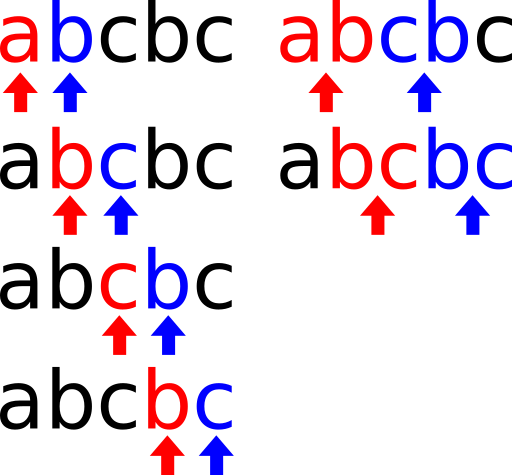
\includegraphics[scale = 0.2]{images/squareFinding}
    \caption{Działanie algorytmu szukającego kwadratów.}
    \label{fig:squareFinding}
\end{figure}

Dla typu gry w którym unikamy nasunięć powstały osobne metody.

\begin{lstlisting}[frame=single]
Subsequence findOverlap(List<Integer> sequence) {
	Subsequence repeatedSequence = null;
	int maxSeqSize = (sequence.size()/2)+1;
	int minSeqSize = 3;
	for(int subSeqSize=minSeqSize; subSeqSize<=maxSeqSize; subSeqSize++) {
		repeatedSequence = compareSubSeqOverlap(subSeqSize, sequence);
		if(repeatedSequence != null) {
			return repeatedSequence;
		}
	}
	return null;
}
\end{lstlisting}

Metoda \textbf{findOverlap}, działa w sposób podobny do metody \textbf{findSquare}. Różnice to inne wartości zmiennych \textbf{maxSeqSize}, \textbf{minSeqSize} oraz metoda wywoływana w pętli.

Do zmiennej \textbf{maxSeqSize} przypisywana jest liczba o jeden większa niż długość sekwencji, ponieważ szukamy nasunięcia, a więc podciągi będą ze sobą dzieliły jeden znak. Wobec tego dla ciągu $S = \{abcabcb\}$, najdłuższy porównywany ciąg będzie długości 4, ponieważ w ostatniej iteracji pętli będziemy ze sobą porównywali podciągi $abca$ oraz $abcb$, które dzielą ze sobą literę $a$.

Wartość zmiennej \textbf{minSeqSize} wynosi 3, ponieważ jest to warunkiem stworzenia nasunięcia.

\begin{lstlisting}[frame=single]

Subsequence compareSubSeqOverlap(int subSeqSize, List<Integer> sequence) {
	List<Integer> left = new ArrayList<>();
	List<Integer> right = new ArrayList<>();
	int comparesFitInSequence = (sequence.size() + 2) - (subSeqSize*2);
	for(int i=0; i<comparesFitInSequence; i++) {
		for(int j =0;j<subSeqSize;j++) {
			left.add(sequence.get(i+j));
			right.add(sequence.get(i+j+subSeqSize-1));
		}
		if(listsAreEqual(left, right)) {
			return new Subsequence(left, i, subSeqSize);
		}
		left.clear();
		right.clear();
	}
	return null;
} 
\end{lstlisting}

Metoda \textbf{compareSubSeqOverlap} również jest analogiczna do metody \textbf{compareSubSeq}. Różni się tutaj wartość zmiennej \textbf{comparesFitInSequence}, jest ona większa o 1, z takiego samego powodu, co zmienna \textbf{maxSeqSize} z metody \textbf{findOverlap}. Różni się również podciąg zapisywany do zmiennej \textbf{right}, w pętli z 6 linii. Pierwszy indeks owego podciągu jest równy indeksowi ostatniego elementu, lewego podciągu, po to by stworzyć nasunięcie.

\begin{figure}[H]
    \centering
    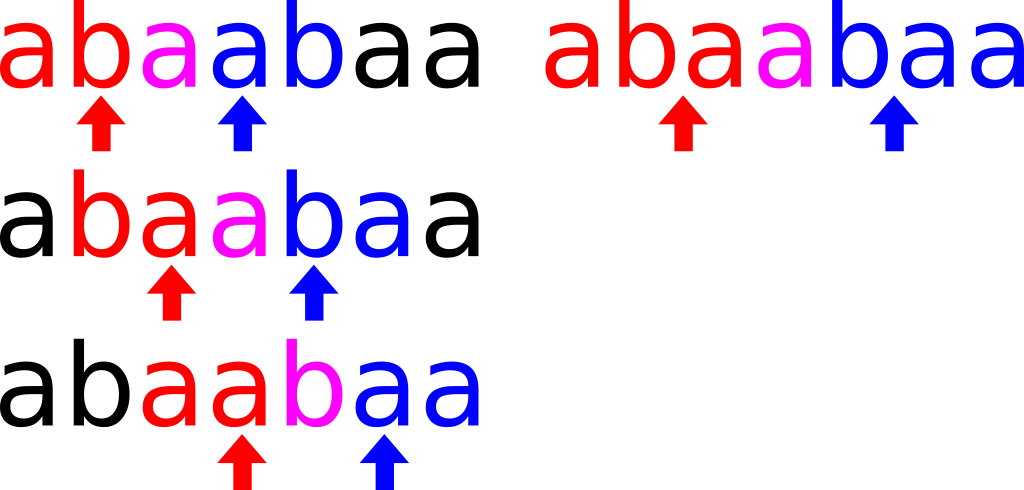
\includegraphics[scale = 0.2]{images/overlapFinding}
    \caption{Działanie algorytmu szukającego nasunięć.}
    \label{fig:overlapFinding}
\end{figure}

\section{Komunikacja z użytkownikiem}
Plik konfiguracyjny nie jest wystarczającym środkiem komunikacji z aplikacjią. W związku z tym, po uruchomieniu programu mamy dostęp do konsoli, służy do wyświetlania jak i wprowadzania treści.

Po uruchomieniu aplikacji w konsoli wypisywane są najważniejsze opcje konfiguracyjne, takie jak poziom budowniczego, poziom malarza oraz lista dostępnych symboli. Jeśli uruchomiliśmy grę w trybie \textbf{humanHuman}, to aplikacja w pierwszej kolejności poprosi nas o indeks. Po wpisaniu indeksu mieszczącego się w przedziale $\in [0,...,n]$, gdy to zrobimy zostaniemy poproszeni o podanie symbolu $\geq 0$ i $< setPower$. W momencie gdy podaliśmy prawidłowe wartości na ekran konsoli wyświetlany zostaje ciąg $S'$, który został utworzony poprzez dodanie do istniejącego ciągu odpowiedniego symbolu. Jeśli w ciągu $S'$ pojawi się kwadrat, na ekran zostanie wyświetlony czas rozgrywki, ilość ruchów jaka została do tej pory wykonana oraz indeksy wraz z symbolami, wspomnianego powtórzenia.

Oto przykład prostej rozgrywki:

\begin{lstlisting}
#> W grze dostepne sa nastepujace liczby: 
0
1
2
 0: { 0 }  1: {   } 
## =============================================================== ##
#> Podaj indeks: 
1
#> Podaj liczbe: 
2
 0: { 0 }  1: { 2 }  2: {   } 
## =============================================================== ##
#> Podaj indeks: 
1
#> Podaj liczbe: 
1
 0: { 0 }  1: { 1 }  2: { 2 }  3: {   } 
## =============================================================== ##
#> Podaj indeks: 
3
#> Podaj liczbe: 
1
 0: { 0 }  1: { 1 }  2: { 2 }  3: { 1 }  4: {   } 
## =============================================================== ##
#> Podaj indeks: 
4
#> Podaj liczbe: 
2
 0: { 0 }  1: { 1 }  2: { 2 }  3: { 1 }  4: { 2 }  5: {   } 
## =============================================================== ##

#> Znaleziono kwadrat:  
 1: { 1 }  2: { 2 }  <->  3: { 1 }  4: { 2 } 

## =============================================================== ##

#> Rozrgrywka trwala 5 ruchow i 20.339 sekund.
\end{lstlisting}
Jeśli uruchomimy rozgrywkę z komputerem, obok wybranego indeksu lub symbolu pojawia się również czas jaki był mu potrzebny na podjęcie decyzji.

\begin{lstlisting}
#> Komputer wybral indeks: 1 	| Czas trwania obliczen: 24.127 s
#> Komputer wybral liczbe: 4 	| Czas trwania obliczen: 0.012 s\end{lstlisting}

By ułatwić późniejszą analizę wszystkie informacje zawarte w konsoli, zapisywane są do nowo utworzonego pliku w katalogu output.

\section{Zachłanny algorytm wyszukiwania symbolu}
Jak zostało wcześniej wspomniane można sterować poziomem inteligencji komputerowych oponentów za pomocą zmiennych konfiguracyjnych. Jeśli ustawimy poziom zagnieżdżeń na 0, algorytm będzie działał zachłannie, wybierając opcje, która jest najatrakcyjniejsza w danym momencie, nie zważając na to, co może wydarzyć się w kolejnej turze. Obrazuje to poniższy algorytm szukający pasującego symbolu na wskazanym wcześniej indeksie.

\begin{lstlisting}[frame=single]
int findRightColorGreedy(List<Integer> sequence, int index, int power) {
		for(int symbol=0;symbol<power; symbol++) {
			sequence.add(index, symbol);
			if(pickProperFind(sequence) == null) {
				sequence.remove(index);
				return symbol;
			} else {
				sequence.remove(index);
			}
		}
		return -1;
	}
\end{lstlisting}

Metoda na wejściu dostaje trzy parametry:
\begin{itemize}
\item sequence - utworzony wcześniej ciąg.
\item index - indeks wybrany przez budowniczoego.
\item power - moc zbioru symboli.
\end{itemize}
Zbiór symboli to kolejne liczby naturalne z przedziału  $\in [0; power-1]$. W 2 linii metody rozpoczyna się pętla, która iteruje po wszystkich dostępnych symbolach. W kolejnej linii symbol dodawany jest do naszego ciągu na podanej pozycji. Metoda pickProperFind z warunku if zależnie od typu gry wywołuje wcześniej opisane metody findSquare lub findOverlap. Jeśli warunek if zostanie spełniony oznacza to, że po dodaniu aktualnego symbolu na danej pozycji nie powoduje stworzenia kwadratu/nasunięcia, algorytm zatem usuwa dodany element z ciągu i zwraca go w linii 6. Jeżeli  okaże się jednak, że dodany symbol tworzy powtórzenie w ciągu, zostaje on również usunięty, a pętla zaczyna się od początku. Metoda zwraca wartość -1 jeśli okaże się, że żaden z symboli nie jest w stanie stworzyć ciągu wolnego od kwadratów/nasunięć.

\section{Zachłanny algorytm wyszukiwania indeksu}
By można było przeprowadzić symulację gry, należy wprowadzić również algorytm budowczniego, starający się znaleźć najmniej atrakcyjny indeks dla malarza. Zachłanny algorytm realizujący to zadanie znajduje się poniżej.

\begin{lstlisting}[frame=single]
int findRightIndexGreedy(List<Integer> sequence, int power) {
	int winner = -1;
	int smallestSymbolSize = power;
	for (int i =0;i<sequence.size()+1;i++) {
		List<Integer> symbols = getFitableColorList(sequence, i);
		if (symbols.size() <= smallestSymbolSize) {
			smallestSymbolSize = symbols.size();
			winner = i;
		}
	}
	return winner;
}
\end{lstlisting}

Algorytm jako parametry, otrzymuje stworzony wcześniej ciąg, oraz moc zbioru symboli. Zmienna winner ustawiona początkowo na -1, reprezentuje indeks, który zostanie zwrócony jako ten, pod którym jest najmniejsza dowolność wyboru symboli, bez tworzenia powtórzeń. Metoda iteruje po każdym indeksie ciągu i zapisuje do listy symbole, po których wstawieniu w dane miejsce nie utworzy się kwadrat/nasunięcie. Następnie w warunku if z 6 linii sprawdzane jest, czy aktualna lista symboli jest mniejsza niż ta, zarejestrowana wcześniej. Jeśli tak, do zmiennej winner zapisany zostaje aktualny indeks.

\section{Algorytm wyszukiwania symbolu z zagnieżdżeniami}
Algorytm zachłanny nie jest wystarczająco sprytny, żeby przeciwstawić się człowiekowi mającemu odrobinę doświadczenia w Longest free word. Wobec tego powstał algorytm nie działający zachłannie, lecz starający się przewidzieć, jakie konsekwencje w kolejnych turach może nieść ze sobą dany wybór.

Poniższy algorytm wprowadza pojęcie punktacji. Podczas jego działania, dla możliwych wyborów nadawane są punkty. Im więcej punktów uzyska dany symbol, tym atrakcyjniejszym staje się on wyborem. Algorytm sprawdza jakie symbole można dodać w predefiniowanym indeksie, następnie iterując w pętli, dodaje każdy z symboli i sprawdza, ile możliwości będzie miał w kolejnej lub kolejnych turach, biorąc pod uwagę wszystkie dostępne indeksy. Każda dodatkowa możliwość to dodatkowy punkt dla wybranego koloru. Sam algorytm składa się z dwóch głownych części: \textbf{findRightColorPredicting} oraz \textbf{simulation}.

\begin{lstlisting}[frame=single]
int findRightColorPredicting(List<Integer> sequence, int index) {
	List<Integer> scoreList = initScoreList(power);
	List<Integer> symbolList = getFitableSymbolList(sequence, index);
	for(int symbol: symbolList) {
		sequence.add(index, symbol);
		simulation(sequence, symbol, scoreList, painterNestingLevel);
		sequence.remove(index);
	}
	return getRandomFromScoreList(scoreList);
}
\end{lstlisting}

Na początku algorytm inicjalizuje listy \textbf{scoreList} oraz \textbf{symbolList}. Tę pierwszą tyloma zerami ile jest w grze dostępnych symboli, drugą natomiast symbolami, jakie możemy wstawić w zdefiniowany przez budowniczego indeks. Linia 4 rozpoczyna pętlę, która iterując po liście \textbf{symbolList}, dodaje jej element, wywołuje metodę \textbf{simulation}, przekazując utworzony \textbf{ciąg}, dodany \textbf{symbol}, \textbf{scoreList} oraz p\textbf{oziom zagnieżdżenia malarza}, po czym usuwa dodany \textbf{symbol} sprawiając, że ciąg pozostaje bez zmian. Na końcu zwraca element, który miał największą liczbę punktów. Jeśli kilka symboli otrzymało ich tyle samo, program wybiera losowy z nich. Dzięki w grze występuje pewna przypadkowość, oraz jest mała szansa na powtórzenie dwóch identycznych rozgrywek przy odpowiednio długim ciągu.

Wewnątrz metody \textbf{simulation} nadawane są punkty, oraz za pomocą rekurencji wykonywana jest symulacja kolejnych iteracji gry.

\begin{lstlisting}[frame=single]
void simulation(List<Integer> sequence, int indexInScoreList, List<Integer> scoreList, int invokes) {
	invokes--;
	for(int j=0;j<sequence.size()+1;j++) {
		List<Integer> symbolList = getFitableSymbolList(sequence, j);
		updateScoreList(scoreList, indexInScoreList, symbolList.size());
		for(int symbol: symbolList) {
			sequence.add(j, symbol);
			if(invokes > 0) {
				simulation(sequence, indexInScoreList, scoreList, invokes);
			}
			sequence.remove(j);
		}
	}
}
\end{lstlisting}

Na początku dekrementowana zostaje ilość zagnieżdżeń na jaką chcemy się zagłębić. Oznacza to, że jeśli poziom zagnieżdżenia ustawiony jest na 1, to metoda \textbf{simulation} zostanie wywołana tylko raz. Pętla z 3 linii iteruje po indeksach pod którymi możliwe jest dodanie symbolu. W 4 linii do listy zapisywane są symbole, które można wcisnąć pod aktualny indeks, nie powodując powtórzenia. Metoda \textbf{updateScoreList} zwiększa ilość punktów symbolu przekazanemu z poprzedniej metody. Ilość punktów jest równa liczbie elementów, zmiennej \textbf{symbolList}. Pętla z 6 linii iterując po liście pasujących symboli, dodaje element, następnie pod warunkiem, że \textbf{invokes} jest większe od 0 wywołuje samą siebie ze zmodyfikowanym ciągiem, tym samym indeksem, który został przekazany na początku, listą punktową oraz pozostałą liczbą wywołań. Na końcu pętli element zostaje usunięty, po to, by ciąg wrócił do pierwotnego stanu.

Algorytm obrazuje poniższa grafika:


\begin{figure}[H]
    \centering
    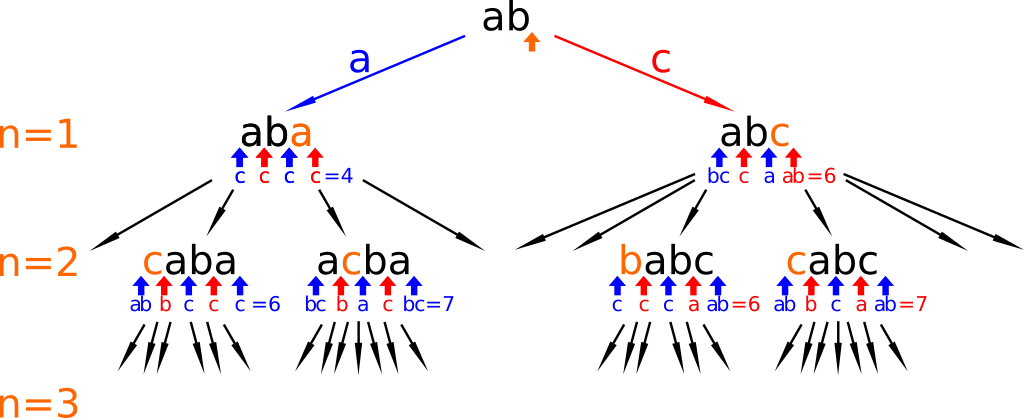
\includegraphics[scale = 0.08]{images/nestingPainter}
    \caption{Działanie algorytmu malarza z zagnieżdżeniami.}
    \label{fig:nestingPainter}
\end{figure}

Mamy ciąg $S = a, b$, budowniczy wybrał indeks 2, czyli malarz wybiera symbol jaki zostanie wstawiony za literką $b$. Typ gry to \textbf{Longest square free word}. Moc zbioru wynosi 3, więc do wyboru są dostępne symbole $a$, $b$, $c$. Wstawienie symbolu $b$ stworzyłoby kwadrat, dlatego algorytm rozważa literki $a$ oraz $c$. Zmienna $n$ jest to poziom zagnieżdżenia algorytmu, natomiast liczby przy pasujących symbolach oznaczają punkty, jakie zostają przypisane symbolowi $a$ lub $c$. 

Już przy pierwszym zagnieżdżeniu widać, że literka $c$ jest atrakcyjniejsza, ponieważ wstawienie jej zapewnia malarzowi więcej możliwości w kolejnych rundach. Jednak sprawdzenie jednego ruchu do przodu nie zawsze jest wystarczające i zdarza się, że z pozoru nieatrakcyjny symbol w perspektywie kolejnych, tur jest najlepszą opcją.

\section{Algorytm wyszukiwania indeksu z zagnieżdżeniami}
Sposób działania algorytmu z zagnieżdżeniami szukającego indeksu, który ma największą szansę na stworzenie powtórzenia, działa na podobnej zasadzie, co algorytm wyszukiwania symbolu. Różnica polega na tym, że w jego pierwszej części, iterujemy po wszystkich dostępnych symbolach, a nie jednym predefiniowanym, oraz punkty nadawane zostają indeksom i zwracamy ten, który uzyska ich najmniej. Druga część algorytmu czyli metoda \textbf{simulation} pozostaje bez zmian.

\begin{lstlisting}[frame=single]
int findRightIndex(List<Integer> sequence) {
	List<Integer> scoreList = initScoreList(sequence.size() + 1);
	for (int i = 0; i<sequence.size() + 1; i++) {
		List<Integer> symbols = getFitableSymbolList(sequence, i);
		for (int symbol : symbols) {
			sequence.add(i, symbol);
			simulation(sequence, i, predictList, builderNestingLevel);
			sequence.remove(i);
		}
	}
	return getRandomMinFromPredict(scoreList);
}
\end{lstlisting}

Na początku metody zainicjalizowana zostaje zmienna scoreList. Do listy dodane zostają zera w ilość odpowiadającej długość ciągu plus jeden, bo właśnie na tylu indeksach możemy dodać nowy element. W 3 linii iterujemy po każdym dostępnym indeksie, natomiast od 4 linii mamy już wszystko to co w algorytmie szukającym symbolu. Na końcu metody zwracany zostaje indeks, który uzyskał najmniej punktów, czyli będzie najmniej atrakcyjny dla malarza. Tak jak poprzednio jeśli istnieje więcej niż jeden indeks z minimalna wartością, element jest wybierany losowo.

\section{Longest square free word z interfejsem graficznym}
Napisałem również wersję gry, w której użytkownik nie korzysta z konsoli, lecz z graficznego interfejsu. W tej odmianie użytkownik za pomocą trzech kolorów ma stworzyć jak najdłuższy ciąg bez kwadratów. Czynności jakie gracz wykonuje to wybranie miejsca, w które zostanie wstawiony element oraz jego kolor. Jeśli w tworzonym ciągu pojawi się kwadrat rozgrywka zostaje przerwana i na ekranie zostają podświetlone powtórzenia składające się na kwadrat. Program zapisuje również najwyższy wynik, który jest równy długości utworzonego ciągu. Algorytm szukający kwadratów nie różni się w żaden sposób od algorytmu z podstawowej wersji gry.

\begin{figure}[H]
    \centering
    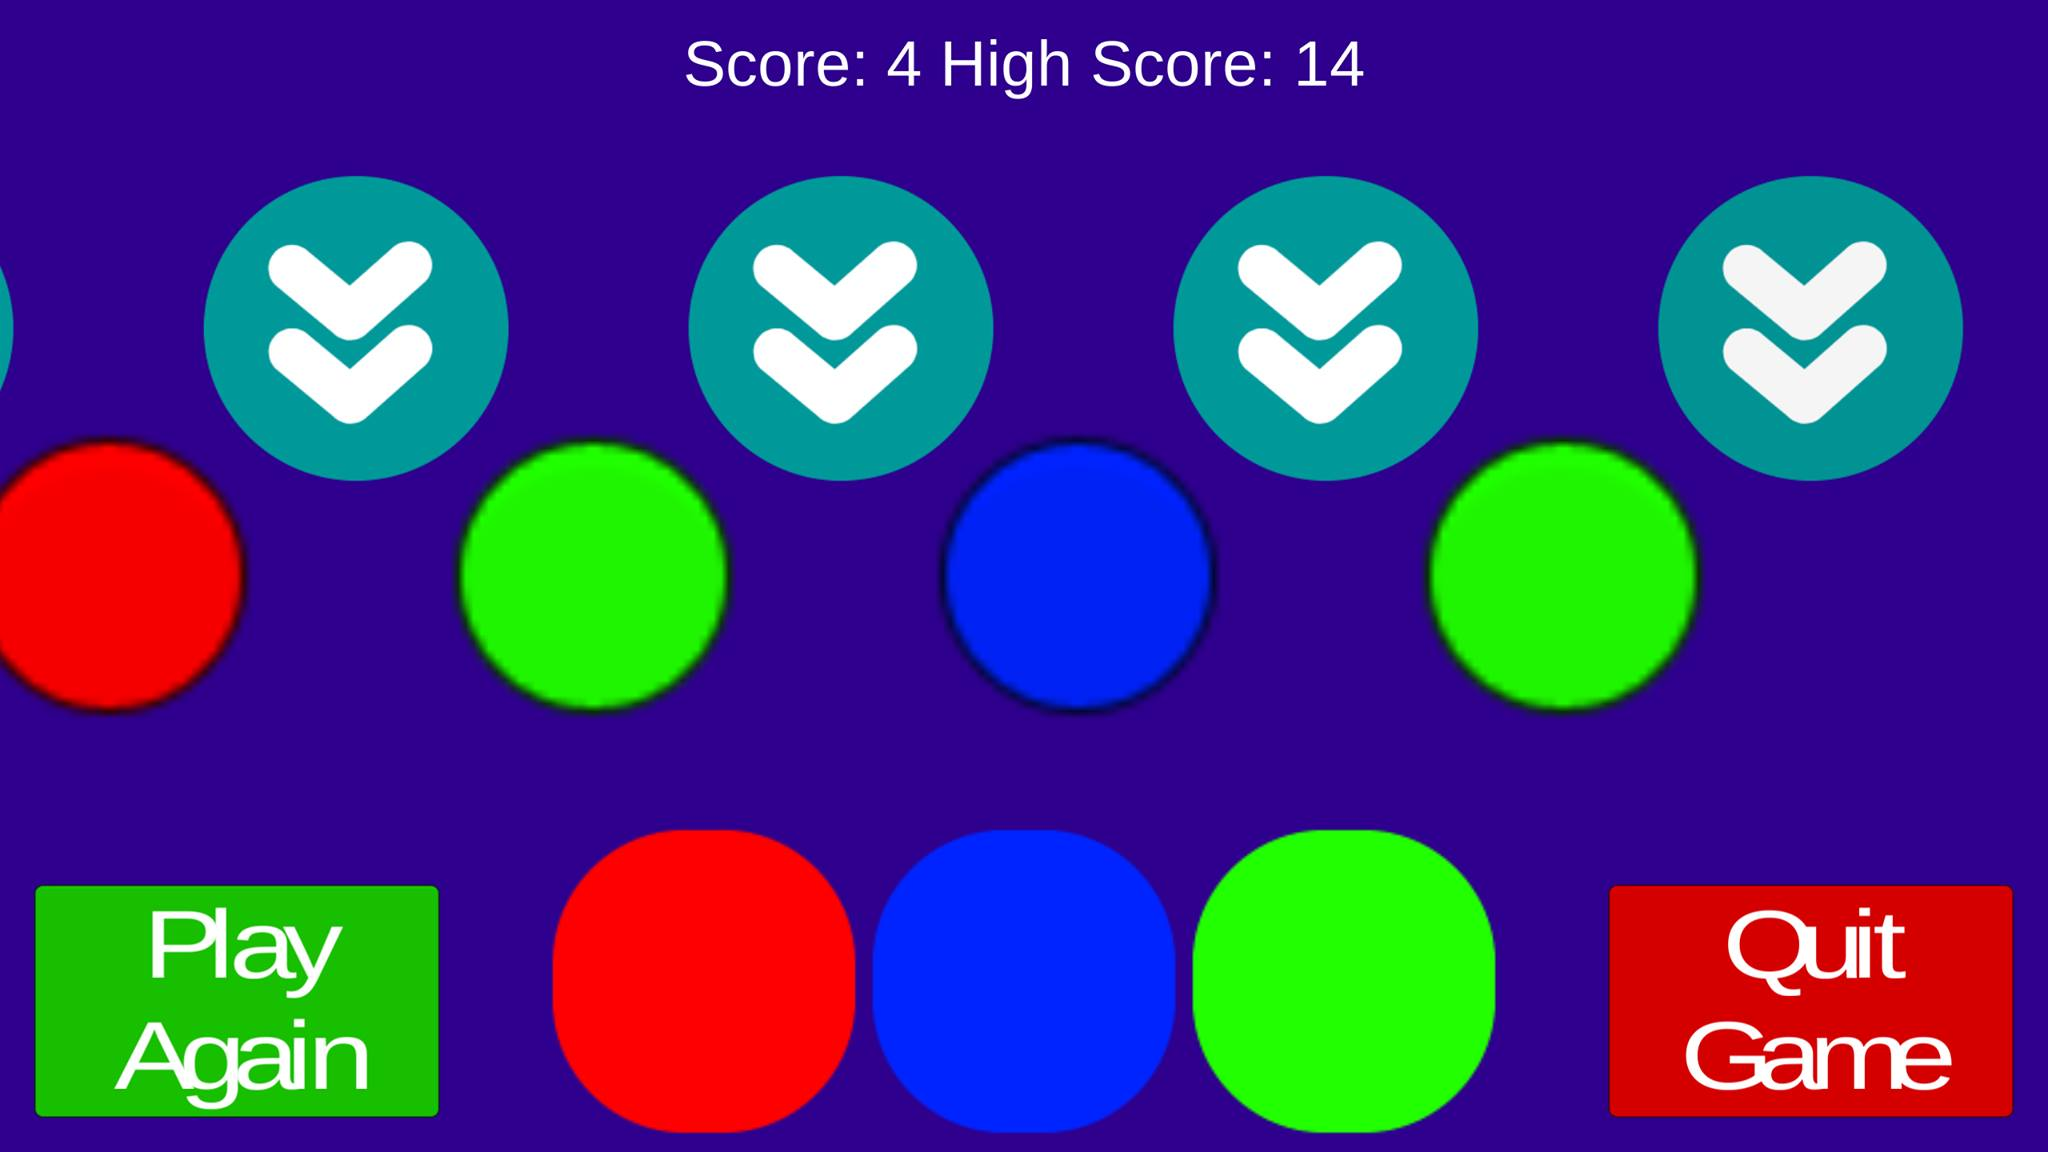
\includegraphics[scale = 0.2]{images/thueMobile}
    \caption{Longest Free Word z interfejsem graficznym}
    \label{fig:thueMobile}
\end{figure}

Aplikacja została napisana na popularnym silniku do tworzenia gier - Unity. Pozwala on kompilować kod programu do plików wykonywalnych, które mogą być uruchamiane w przeglądarkach, na komputerach osobistych, konsolach i telefonach komórkowych. W tym przypadku pod uwagę brane były głównie telefony komórkowe, o czym może świadczyć wielkość przycisków i mała ilość wyświetlonych szczegółów.


\chapter{Analiza symulowanych potyczek} 
Dobrym sposobem by poznać aplikację jest jej uruchomienie. Jeszcze lepszym, przeprowadzenie jej analizy oraz zobrazowanie wyników za pomocą wykresów i tabel. Rozdział ten poświęcony jest badaniu działania aplikacji Longest Free Word. Badania skupiają się na wariancie aplikacji opierającym się na tworzeniu ciągu bez kwadratów. Wszystkie testy uruchomione były na maszynie zdalnej z systemem operacyjnym Ubuntu 15.10, procesorem 2,6 Ghz Intel Core i7, pamięcią ram 16 GB 1600 MHz DDR3 i dyskiem SSD.

\section{Ilość symboli potrzebna na rozgranie partii}
Długość gry zależna jest od dwóch czynników. Ustawionego poziomu zagnieżdżenia i ilości dostępnych symboli. Thue w swoim twierdzeniu \cite{repetition}, udowodnił, że jesteśmy w stanie stworzyć nieskończenie długi ciąg bez kwadratów mając do dyspozycji 3 symbole. Sytuacja zmienia się, gdy ciąg tworzony jest przez dwóch oponentów, z których jeden stara się utworzyć kwadrat. Nawet używając zachłannego algorytmu w przypadku budowniczego i algorytmu z zagnieżdżeniami 7 poziomu dla malarza, rozgrywka zawsze trwała będzie maksymalnie 5 ruchów. 

Dla 4 symboli, również nie jest możliwe rozegranie partii dłuższej niż 10 ruchów. Przy zachłannym algorytmie budowniczego, malarz jest w stanie utworzyć ciąg długości 10. Jeśli algorytm budowniczego używa zagnieżdżeń, liczba ta zmniejsza się do 7.

\begin{table}[H]
    \centering
	\begin{tabular}{|l|l|l|l|} \hline
	Ilość symboli & Poziom malarza & Poziom budowniczego & Długość rozgrywki \\ \hline
	$3$ & $\geq 0$ & $\geq 0$ & $5$ ruchów\\ \hline
	$4$ & $0$ & $0$ & $7$ ruchów\\ \hline
	$4$ & $\geq 1 $ & $\geq 1$ & $7$ ruchów\\ \hline
	$4$ & $0$ & $\geq 1$ & $10$ ruchów\\ \hline
	\end{tabular}
	\caption{Maksymalna ilość ruchów w stosunku do ilości dostępnych symboli.}
	\label{fig:maxGameLength}
\end{table}

Jak widać w tabeli \ref{fig:maxGameLength}, przy alfabecie o mocy 4, malarz poziomu zerowego lepiej radzi sobie  od malarza poziomu pierwszego. Dowodzi to tego, że taktyka wykorzystująca zagnieżdżenia nie jest doskonała i nie zawsze jest najlepszą opcją. Pozostałe warianty nie zostały przedstawione, gdyż rozgrywka w ich przypadku nie skutkowała stałym wynikiem. Oznacza to, że taktyka budowniczego nie była wystarczająco dobra by za każdym razem pokonać malarza w takiej samej ilości ruchów.


Dopiero rozgrywka na 5 symbolach daje algorytmom pole do popisu, bowiem w przeprowadzonych badaniach, zależnie od ustawionych poziomów, trwała ona od 11 do conajmniej 236 ruchów.

Używanie zachłannego algorytmu malarza przy alfabecie pięcioelementowym,  nie skutkuje zbyt długą grą. Niezależnie od poziomu budowniczego, kwadrat pojawi się zawsze po wspomnianym 11 kroku. Jednak podczas prób, gdy malarz miał ustawiony poziom zagnieżdżenia równy 1, a budowniczy działał zachłannie, rozgrywka trwała od 44 do 236 tur. Średnia arytmetyczna wyciągnięta z ilości ruchów wyniosła 133.83

\begin{table}[H]
    \centering
	\begin{tabular}{|l|l|l|} \hline
	Ilość symboli & Ilość ruchów & Czas trwania \\ \hline
	5 & 44 & 0.1 s.\\ \hline
	5 & 56 & 0.4 s.\\ \hline
	5 & 81 & 2.4 s.\\ \hline
	5 & 88 & 4.3 s.\\ \hline
	5 & 100 & 7.6 s.\\ \hline
	5 & 102 & 7.3 s.\\ \hline
	5 & 163 & 1 min. 27 s. \\ \hline
	5 & 171 & 1 min. 48 s. \\ \hline
	5 & 173 & 1 min. 59 s. \\ \hline
	5 & 193 & 4 min. \\ \hline
	5 & 199 & 3 min. 38 s.\\ \hline
	5 & 236 & 8 min. 51 s. \\ \hline
	\end{tabular}
	\caption{Podsumowanie badań dla budownieczego poziomu 0 i malarza poziomu 1.}
	\label{fig:builder0Painter1Table}
\end{table}


Przy poziomie budowniczego i malarza ustawionym na 1, podczas 10 prób rozgrywka trwała od 30 do 213 ruchów. Średnia arytmetyczna obliczona na podstawie rozgrywek wynosi 96.9, a więc jest o 37.23 niższa niż, gdy budowniczy używał algorytmu zachłannego. 

\begin{table}[H]
    \centering
	\begin{tabular}{|l|l|l|} \hline
	Ilość symboli & Ilość ruchów & Czas trwania \\ \hline
	5 & 30 & 1.2 s. \\ \hline	
	5 & 42 & 5.1 s. \\ \hline
	5 & 45 & 11 s. \\ \hline	
	5 & 47 & 7.8 s. \\ \hline
	5 & 73 & 1 min. 17 s. \\ \hline
	5 & 104 & 9 min. 38 s. \\ \hline
	5 & 114 & 29 min. 29 s. \\ \hline
	5 & 134 & 1 godz. 30 min. 27 s.  \\ \hline
	5 & 178 & 5 godz. 11 min. 22 s. \\ \hline
	5 & 202 & 9 godz. 42 min. 15 s. \\ \hline
	5 & 213 & 13 godz. 04 min. 35 s. \\ \hline
	\end{tabular}
	\caption{Podsumowanie badań dla budownieczego i malarza poziomu 1.}
	\label{fig:builder1Painter1Table}
\end{table}


Obecne zasoby sprzętowe i czasowe sprawiły, że malarz poziomu 2 okazał się niepokonany w walce z budowniczym poziomu 0. Przy ponad 10 próbach ani razu nie był zmuszony do stworzenia kwadratu w rozgrywkach trwających $\leq 220$ tur i około 26 godzin.





\section{Pomiary czasów potrzebnych na podjęcie decyzji}
Nieodłącznym elementem analizy działania aplikacji jest badanie czasu w jakim wykonuje ona swoje algorytmy. Nie inaczej jest w przypadku Longest Free Word. Najkrótrzy zbadany czas decyzji algorytmu wyniósł 0.001 sekundy, najdłuższy natomiast około 2 godzin. Czas potrzebny na decyzję jest tym dłuższy im dłuższy jest stworzony do tej pory ciąg. Naturalnie więc, na początku rozgrywki algorytm będzie działał szybko, lecz w raz z rozwojem potyczki będzie zwalniał. Zależność tą można zaobserwować na wykresie \ref{fig:builder0painter1}. Widoczne odchylenia to prawdopodobnie efekt działania innego procesu działającego na tej samej maszynie.

\begin{figure}[H]
    \centering
    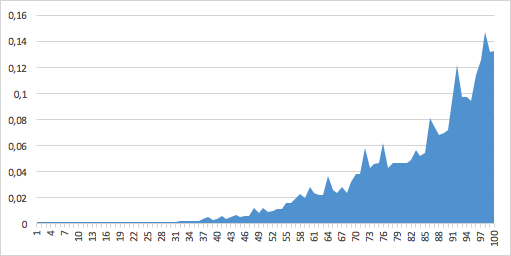
\includegraphics[scale = 0.7]{images/timeBuilder0Painter1}
    \caption{Ilość sekund potrzebna na podjęcie decyzji jako budowniczy przy poszczególnych długościach ciągu. Budowniczy: 0, Malarz: 1.}
    \label{fig:builder0painter1}
\end{figure}

Warto zauważyć jak ogromne różnice w wydajności istnieją pomiędzy poziomami zagnieżdżenia algorytmów.

Przy zagnieżdżeniu ustawionym na 2, dla ciągu długości 100 wyliczenie odpowiedniej decyzji zajęło około 170 razy więcej czasu niż przy zagnieżdżeniu równym 1. Różnice zobrazowane zostały na wykresach \ref{fig:builder1painter1} i \ref{fig:builder2painter1}.

\begin{figure}[h]
    \centering
    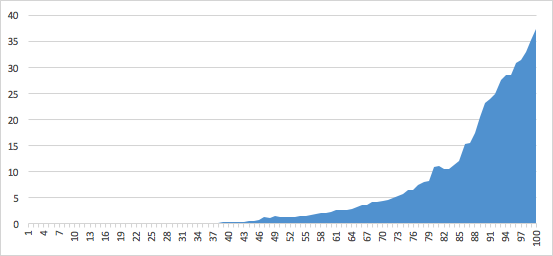
\includegraphics[scale = 0.7]{images/timeBuilder1Painter1}
    \caption{Ilość sekund potrzebna na podjęcie decyzji jako budowniczy przy poszczególnych długościach ciągu. Budowniczy: 1, Malarz: 1.}
    \label{fig:builder1painter1}
\end{figure}

\begin{figure}[H]
    \centering
    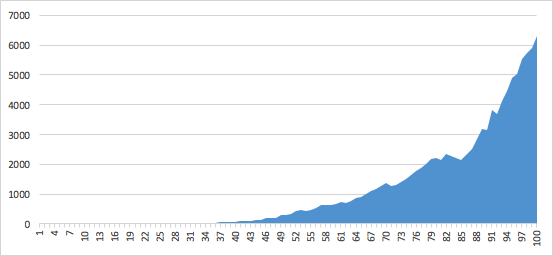
\includegraphics[scale = 0.7]{images/timeBuilder2Painter1}
    \caption{Ilość sekund potrzebna na podjęcie decyzji jako budowniczy przy poszczególnych długościach ciągu. Budowniczy: 2, Malarz: 1.}
    \label{fig:builder2painter1}
\end{figure}



Odrobinę inaczej wyglądają analogiczne wykresy dla malarza. Algorytm malarza z zagnieżdżeniami symuluje dodawanie kolejnych symboli w wyznaczonym indeksie, jednak jeżeli w danym miejscu da się wstawić tylko jeden symbol, to przeprowadzi mniej symulacji, niż jeśli dałoby się tam wstawić pięć symboli. Dzięki tej zależności na wykresie można zauważyć, przy których ruchach malarz jest w opałach, a przy których ma dostępnych wiele opcji.

Wykres \ref{fig:painter1builder0} przedstawia wzloty i spadki czasu trwania algorytmu. Jak widać zachłanny algorytm budowniczego cyklicznie redukuje liczbę opcji malarza.

\begin{figure}[h]
    \centering
    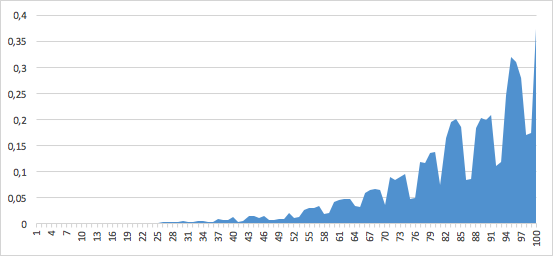
\includegraphics[scale = 0.7]{images/timePainter1Builder0}
    \caption{Ilość sekund potrzebna na podjęcie decyzji jako malarz przy poszczególnych długościach ciągu. Budowniczy: 0, Malarz: 1.}
    \label{fig:painter1builder0}
\end{figure}

Jeśli przeanalizujemy wykres \ref{fig:painter1builder2} zauważymy, że podczas rozgrywki ze sprytniejszym algorytmem budowniczego, krzywe są o wiele bardziej spiczaste, co oznacza, że jest to trudna rozgrywka dla malarza, która ostatecznie kończy się w 82 ruchu.

Ponownie możemy porównać ze sobą czasy podejmowania decyzji dla algorytmu z zagnieżdżeniem 1 poziomu na wykresie \ref{fig:painter1builder2}, oraz 2 poziomu na wykresie \ref{fig:painter2builder0}. Wykonanie ruchu, dla ciągu długości 79 pierwszemu algorytmowi zajęło $0.061$ sekundy, natomiast temu bardziej złożonemu $17.711$. Zatem w tym konkretnym ruchu algorytm z zagnieżdżeniem o $1$ większym decydował się około $290$ razy dłużej.

\begin{figure}[h]
    \centering
    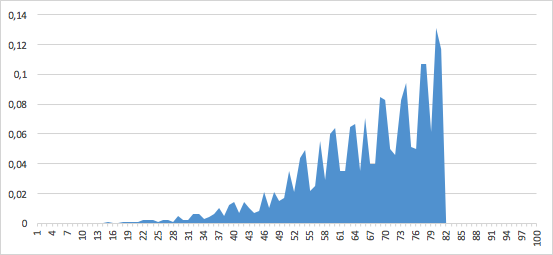
\includegraphics[scale = 0.7]{images/timePainter1Builder2}
    \caption{Ilość sekund potrzebna na podjęcie decyzji jako malarz przy poszczególnych długościach ciągu. Budowniczy: 2, Malarz: 1.}
    \label{fig:painter1builder2}
\end{figure}

\begin{figure}[h]
    \centering
    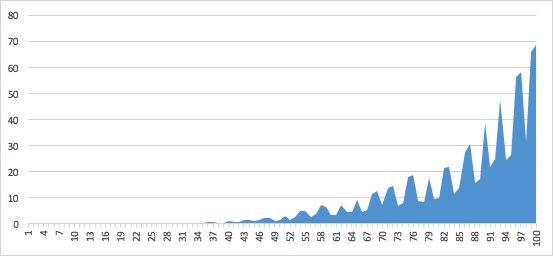
\includegraphics[scale = 0.7]{images/timePainter2Builder0}
    \caption{Ilość sekund potrzebna na podjęcie decyzji jako malarz przy poszczególnych długościach ciągu. Budowniczy: 0, Malarz: 2.}
    \label{fig:painter2builder0}
\end{figure}


\section{Porównanie zachowań algorytmu z zagnieżdżeniami i bez zagnieżdżeń}
Jeśli przyjrzymy się dokładnie działaniu zachłannego algorytmu wyszukiwania indeksu, to bez trudu zauważymy, że w początkowej fazie gry, kiedy malarz ma dużą swobodę w wybieraniu elementów, indeks, który jest wybierany to w przeważającej większości ostatni indeks ciągu. Spowodowane jest to tym, że indeksy $0$ oraz $n+1$, otoczone są elementami tylko z lewej lub prawej strony, dzięki temu malarz ma na nich do wyboru większą gamę symboli. Na reszcie indeksów zazwyczaj dostępne jest tyle samo symboli, zwracany jest więc ostatni z nich, dokładnie tak jak zostało to zaimplementowane. Taktyka tego typu została przeze mnie nazwana \textit{taktyką iteracyjną} i nie jest zbyt emocjonująca. Jeśli nie mamy zbyt dużej puli symboli do wyboru, to po pewnym czasie następuje wyłamanie się z tego stylu gry. Wyłamanie pojawia się zawsze w momencie, gdy budowniczy znajduje indeks z mniejszą ilością możliwości. 

Przeprowadzone przeze mnie badania, przy mocy zbioru symboli równym 5, oraz poziomie malarza równym, 1 wykazały, że w przeciągu kilku kroków od pierwszego znalezienia indeksu, pod którym dostępne są dwa symbole, pojawia się indeks pod którym dostępny jest tylko jeden symbol. Nie wykryłem natomiast korelacji, pomiędzy pierwszym wyłamaniem się z \textit{taktyki iteracyjnej}, a długością rozgrywki. 
 
\begin{figure}[H]
    \centering
    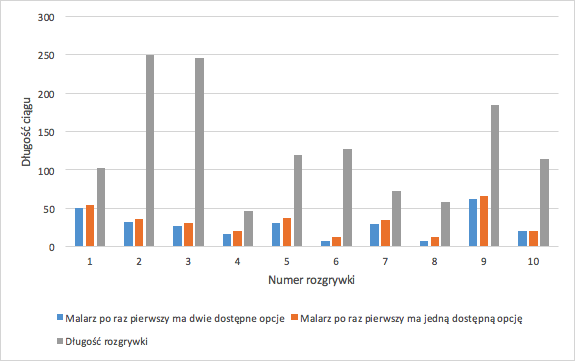
\includegraphics[scale = 0.7]{images/builder0efficiency}
    \caption{Stosunek pierwszego wystąpienia indeksu z dwoma dostępnymi elementami, do pojawienia się indeksu z jednym dostępnym elementem i długości rozgrywki.}
    \label{fig:builder0Efficiency}
\end{figure}

Ciężko jest dopatrzyć się podobnej cykliczności w algorytmie z zagnieżdżeniami. Algorytm ten skupia się raczej na grupie indeksów będących obok siebie. Wykres \ref{fig:buildersPickedIndexes} przedstawia rozkład wybieranych indeksów przez oba algorytmy. Rozgrywki nie trwały więcej niż 115 ruchów, na rysunku można zaobserwować, że najczęściej wybierane indeksy przez algorytm z zagnieżdżeniami należały do zbioru $\leq 27$. Natomiast indeksy wybierane przez algorytm zachłanny, są w miarę równomiernie rozłożone przez wszystkie indeksy. Ponadto, mimo wyłamania się z wcześniej wspomnianej \textit{taktyki iteracyjnej}, algorytm zachłanny w dalszym ciągu działa cyklicznie, wybierając indeksy po zero, jeden lub pięć razy.

\begin{figure}[h]
    \centering
    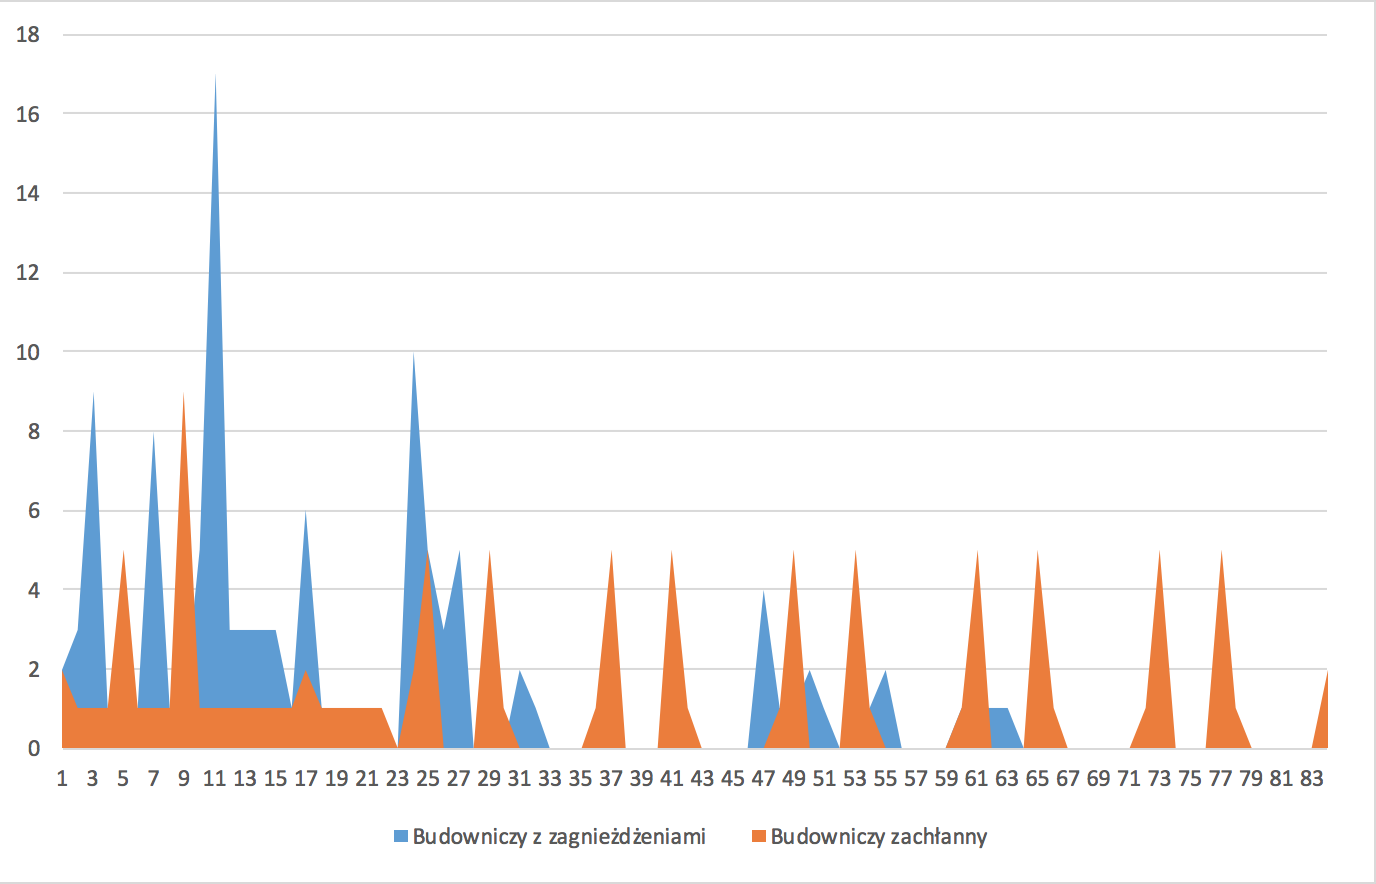
\includegraphics[scale = 0.6]{images/buildersPickedIndexes}
    \caption{Porównanie rozkładu wybieranych indeksów przez budowniczego z zagnieżdżeniami oraz budowniczego zachłannego.}
    \label{fig:buildersPickedIndexes}
\end{figure}

% zakończenie
\summary
Partl~\cite{pa} przedstawi\l \ldots
Możliwości, jakie stoją przed archiwum prac magisterskich opartych na
XML-u, są ograniczone jedynie czasem, jaki należy poświęcić na pełną
implementację systemu. Nie ma przeszkód technologicznych do stworzenia
co najmniej równie doskonałego repozytorium, jak ma to miejsce w
przypadku ETD. Jeżeli chcemy w pełni uczestniczyć w rozwoju nowej ery
informacji, musimy szczególną uwagę przykładać do odpowiedniej
klasyfikacji i archiwizacji danych. Sądzę, że język XML znacznie to
upraszcza.

% załączniki (opcjonalnie):
\appendix
\chapter{Tytuł załącznika jeden}

Treść załącznika jeden.

\chapter{Tytuł załącznika dwa}

Treść załącznika dwa.

% literatura (obowiązkowo):
\bibliographystyle{unsrt}
Axel Thue's papers on repetitions in words:
a translation
\begin{thebibliography}{99}

\bibitem{repetition} Axel Thue's papers on repetitions in words: a translation, July 1994.

\bibitem{narad} N. Rampersad Overlap-Free Words and Generalizations, June 2008.

\bibitem{prouhet} M. E. Prouhet. Memoire sur Quelques Relations Entre les Puissances des Nombres, January 1851.

\bibitem{carpi} A. Carpi, On the size of a squarefree morphism on a three letter alphabet, June 1983.

\bibitem{first} A. Kündgen and M. J. Pelsmajer, Nonrepetitive colorings of graphs of bounded treewidth, August 2007.

\bibitem{thueonline2} J. Grytczuk, J. Kozik, P. Micek, New approach to nonrepetitive sequences, November 2011.

\bibitem{second} J. Barát, P. P. Varjú. On square-free vertex colorings of graphs, April 2006.

\bibitem{thueonline} J. Grytczuk, P. Szafruga, M. Zmarz, Online version of the theorem of Thue, April 2012.

\end{thebibliography}

% spis tabel (jeżeli jest potrzebny):
\listoftables

% spis rysunków (jeżeli jest potrzebny):
\listoffigures

\oswiadczenie

\end{document}
